% Large-field DFS with Upside CVaR: 10-minute progress presentation.
% Based on ams_553_slides_edited.pdf (group edits), trimmed for time.
%
% Build from this folder:   latexmk -pdf slides_10min.tex
% Figures come from results/figures/ and presentation/figures/.
%
% Timing guide (10 minutes, 12 slides):
%   1  Title ................................ 0:15   Marcus
%   2  Large-field DFS ...................... 0:45   Marcus
%   3  Points != payout ..................... 1:00   Marcus
%   4  Haugh & Singal, and what we change ... 1:00   Benjamin
%   5  Simulation pipeline .................. 1:00   Benjamin
%   6  Why Upside CVaR (skewness) ........... 1:00   Benjamin
%   7  Result 1: simulator matches theory ... 0:45   Alex
%   8  Result 2: field-aware upside ......... 1:00   Alex
%   9  Result 3: over-fitting ............... 1:00   Alex
%  10  Result 4: importance sampling ........ 0:45   Alex
%  11  Next steps ........................... 1:00   Marcus
%  12  Takeaways / Questions ................ 0:30   Marcus
%                                             -----
%                                             ~10:00

% Shared styling for slides.tex and backup.tex.

\documentclass[aspectratio=169,11pt]{beamer}

\usepackage[T1]{fontenc}
\usepackage{lmodern}
\usepackage{amsmath,amssymb}
\usepackage{booktabs}
\usepackage{tikz}
\usetikzlibrary{arrows.meta,positioning,fit}

\graphicspath{{figures/}{../results/figures/}}

% ------------------------------------------------------------------ appearance
\definecolor{navy}{RGB}{23,50,94}
\definecolor{accent}{RGB}{31,119,180}
\definecolor{good}{RGB}{44,160,44}
\definecolor{warn}{RGB}{214,39,40}
\definecolor{soft}{RGB}{240,244,250}
\setbeamercolor{frametitle}{fg=navy}
\setbeamercolor{title}{fg=navy}
\setbeamercolor{structure}{fg=accent}
\setbeamercolor{block title}{bg=navy,fg=white}
\setbeamercolor{block body}{bg=soft}
\setbeamerfont{frametitle}{series=\bfseries,size=\large}
\setbeamertemplate{navigation symbols}{}
\setbeamertemplate{itemize items}[circle]
\setbeamertemplate{blocks}[rounded][shadow=false]
\setbeamertemplate{footline}{%
  \hfill\usebeamercolor[fg]{structure}\scriptsize\insertframenumber\,/\,\inserttotalframenumber\hspace{1em}\vspace{0.6em}}
\AtBeginSection[]{%
  \begin{frame}[plain,noframenumbering]
    \centering\vfill
    {\Large\bfseries\color{navy}\insertsectionnumber.\ \insertsection}\par\vfill
  \end{frame}}

\newcommand{\E}{\mathbb{E}}
\newcommand{\hl}[1]{\textcolor{accent}{\textbf{#1}}}
\newcommand{\ucvar}{\operatorname{U\text{-}CVaR}}
\newcommand{\bigstat}[2]{%
  \begin{minipage}[t]{\linewidth}\centering
    {\LARGE\bfseries\color{navy}#1}\par\vspace{0.3em}
    {\footnotesize #2\par}
  \end{minipage}}


\title{Playing for the Top 0.1\,\%}
\subtitle{Simulating large-field Daily Fantasy Sports contests\\
  and building lineups with Upside CVaR}
\author{Benjamin Minkin \and Marcus Minutello \and Alex Dolce}
\institute{AMS 553 / CSE 529: Simulation and Modeling \quad (work in progress)}
\date{}

\begin{document}

% ====================================================================== 1
\begin{frame}[plain]
  \titlepage
\end{frame}

% ====================================================================== 2
\begin{frame}{Large-field DFS: draft 9 players, beat hundreds of thousands of strangers}
  To play DraftKings' NFL Millionaire Maker, each entry picks a QB, 2 RB, 3 WR, a TE, a
  FLEX (RB/WR/TE) and a D/ST under a \$50{,}000 salary cap, where each player's cost
  reflects their expected points.
  \vspace{1.6em}

  \begin{columns}[t]
    \begin{column}{0.24\textwidth}
      \bigstat{100,000+}{entries every week}
    \end{column}
    \begin{column}{0.24\textwidth}
      \bigstat{30\,\%}{of the prize pool goes to the winning entry ($\approx$ top 0.001\,\%)}
    \end{column}
    \begin{column}{0.24\textwidth}
      \bigstat{\$1 million}{grand prize for first place}
    \end{column}
    \begin{column}{0.24\textwidth}
      \bigstat{$-15\,\%$}{average return: the house keeps a 15\,\% rake}
    \end{column}
  \end{columns}
  \vfill
  {\scriptsize\color{navy} Payouts are top-heavy: to win big you need an exceptionally
  high-scoring week.\par}
\end{frame}

% ====================================================================== 3
\begin{frame}{Maximizing expected points $\neq$ maximizing expected payout}
  \begin{columns}[t]
    \begin{column}{0.32\textwidth}
      \begin{block}{You need a boom}
        Lineups optimized for expected points land far below the winning line, so we
        want a high \emph{best case}, not just a high average.
      \end{block}
    \end{column}
    \begin{column}{0.32\textwidth}
      \begin{block}{Stacking adds upside}
        A quarterback and his own receivers rise and fall together. That correlation adds
        variance, and variance produces winning weeks.
      \end{block}
    \end{column}
    \begin{column}{0.32\textwidth}
      \begin{block}{The field sets the bar}
        The winning score depends on whom everyone else drafted. A popular player who
        booms lifts the whole field; an unpopular one lifts only you.
      \end{block}
    \end{column}
  \end{columns}
  \vspace{1.5em}
  \textbf{Our question:} can a lineup chosen for its \hl{upper-tail average} (Upside CVaR)
  beat the field, and lineups built for expected points, by a statistically significant
  margin?
\end{frame}

% ====================================================================== 4
\begin{frame}{Building on Haugh \& Singal (2019), and what we change}
  \centering\small
  \begin{tabular}{@{}p{0.17\textwidth}p{0.37\textwidth}p{0.40\textwidth}@{}}
    \toprule
    & \textbf{Haugh \& Singal} & \textbf{Us} \\
    \midrule
    Player points & Multivariate normal
      & Gaussian copula, \hl{lognormal} (right-skewed) \\[2pt]
    Opponents & Dirichlet ownership, QB--WR stacking, acceptance--rejection
      & Same (their Algorithm 1), plus 20\,\% optimizer ``sharks'' \\[2pt]
    Candidates & Lineup MILP, mean--variance over a grid of $\lambda$
      & Same MILP, plus one optimal lineup per scenario \\[2pt]
    Pick the best & Monte Carlo, mean--variance vs.\ the winning score
      & \hl{Upside CVaR} vs.\ the simulated top-0.1\,\% score \\[2pt]
    Rare-event estimates & Crude Monte Carlo
      & \hl{Importance sampling} (tested; inside selection is next) \\
    \bottomrule
  \end{tabular}
  \vfill
  {\footnotesize Their result: modeling opponents raised expected P\&L about 4$\times$ in
  top-heavy contests over the 2017 NFL season.\par}
  {\scriptsize M.\,B. Haugh and R. Singal, \emph{How to Play Fantasy Sports Strategically
  (and Win)}, 2019.\par}
\end{frame}

% ====================================================================== 5
\begin{frame}{Three simulation stages, then pick a lineup for its upside}
  \centering
  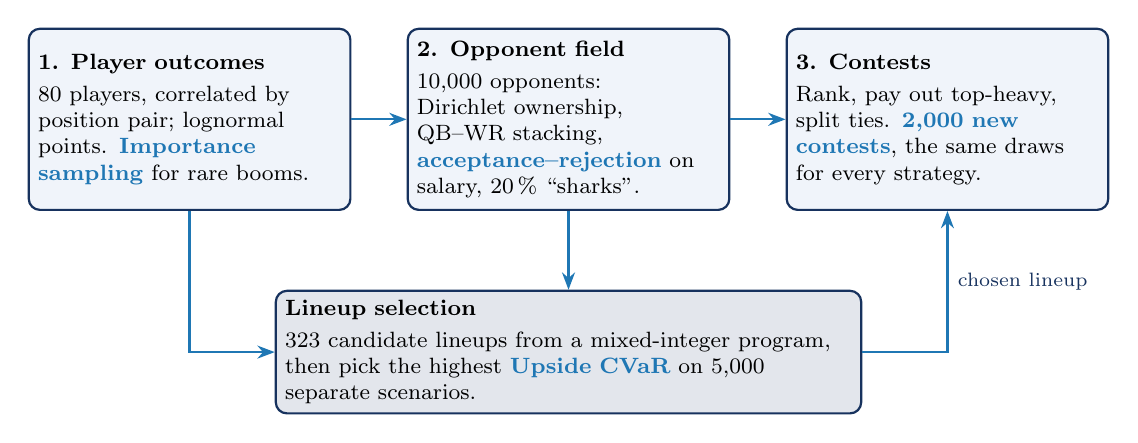
\begin{tikzpicture}[
      box/.style={draw=navy,thick,rounded corners,fill=soft,text width=3.85cm,
                  minimum height=2.3cm,align=left,font=\footnotesize,
                  execute at begin node={\hyphenpenalty=10000\exhyphenpenalty=10000}},
      sel/.style={draw=navy,thick,rounded corners,fill=navy!12,text width=7.2cm,
                  align=left,font=\footnotesize,
                  execute at begin node={\hyphenpenalty=10000\exhyphenpenalty=10000}},
      flow/.style={-{Stealth[length=2.2mm]},thick,accent}]
    \node[box] (s1) {\textbf{1. Player outcomes}\\[2pt]
      80 players, correlated by position pair; lognormal points.
      \hl{Importance sampling} for rare booms.};
    \node[box,right=0.7cm of s1] (s2) {\textbf{2. Opponent field}\\[2pt]
      10{,}000 opponents: Dirichlet ownership, QB--WR stacking,
      \hl{acceptance--rejection} on salary, 20\,\% ``sharks''.};
    \node[box,right=0.7cm of s2] (s3) {\textbf{3. Contests}\\[2pt]
      Rank, pay out top-heavy, split ties. \hl{2{,}000 new contests}, the same draws for
      every strategy.};
    \draw[flow] (s1) -- (s2);
    \draw[flow] (s2) -- (s3);
    \node[sel,below=1.0cm of s2] (opt) {\textbf{Lineup selection}\\[2pt]
      323 candidate lineups from a mixed-integer program, then pick the highest
      \hl{Upside CVaR} on 5{,}000 separate scenarios.};
    \draw[flow] (s1.south) |- (opt.west);
    \draw[flow] (s2.south) -- (opt.north);
    \draw[flow] (opt.east) -| node[pos=0.75,right,font=\scriptsize,text=navy]{chosen lineup} (s3.south);
  \end{tikzpicture}
  \vfill
  {\small Generation, selection and testing each use their own random seed:
  we never grade a lineup on the scenarios that picked it.\par}
\end{frame}

% ====================================================================== 6
\begin{frame}{Why Upside CVaR: fantasy scores are skewed}
  \vspace{-0.6em}
  \[
    \ucvar_\alpha(X) = \E\big[X \mid X \ge q_\alpha(X)\big]
    \approx \frac{1}{k}\sum_{s \in \text{top } k} X_s
  \]
  \vspace{-0.8em}
  \begin{columns}[c]
    \begin{column}{0.40\textwidth}
      \begin{itemize}
        \small
        \setlength\itemsep{0.45em}
        \item \textbf{Paper:} under normality, mean and variance fix the tail, so
          mean--variance is enough
        \item \textbf{Real scores are skewed:} same mean and variance, different upper
          tail
        \item \hl{Field-aware:} $X_s = w^\top\delta_s - G_{(0.1\%),s}$, our score minus the
          top-0.1\,\% score in the \emph{same} contest
      \end{itemize}
    \end{column}
    \begin{column}{0.58\textwidth}
      \centering
      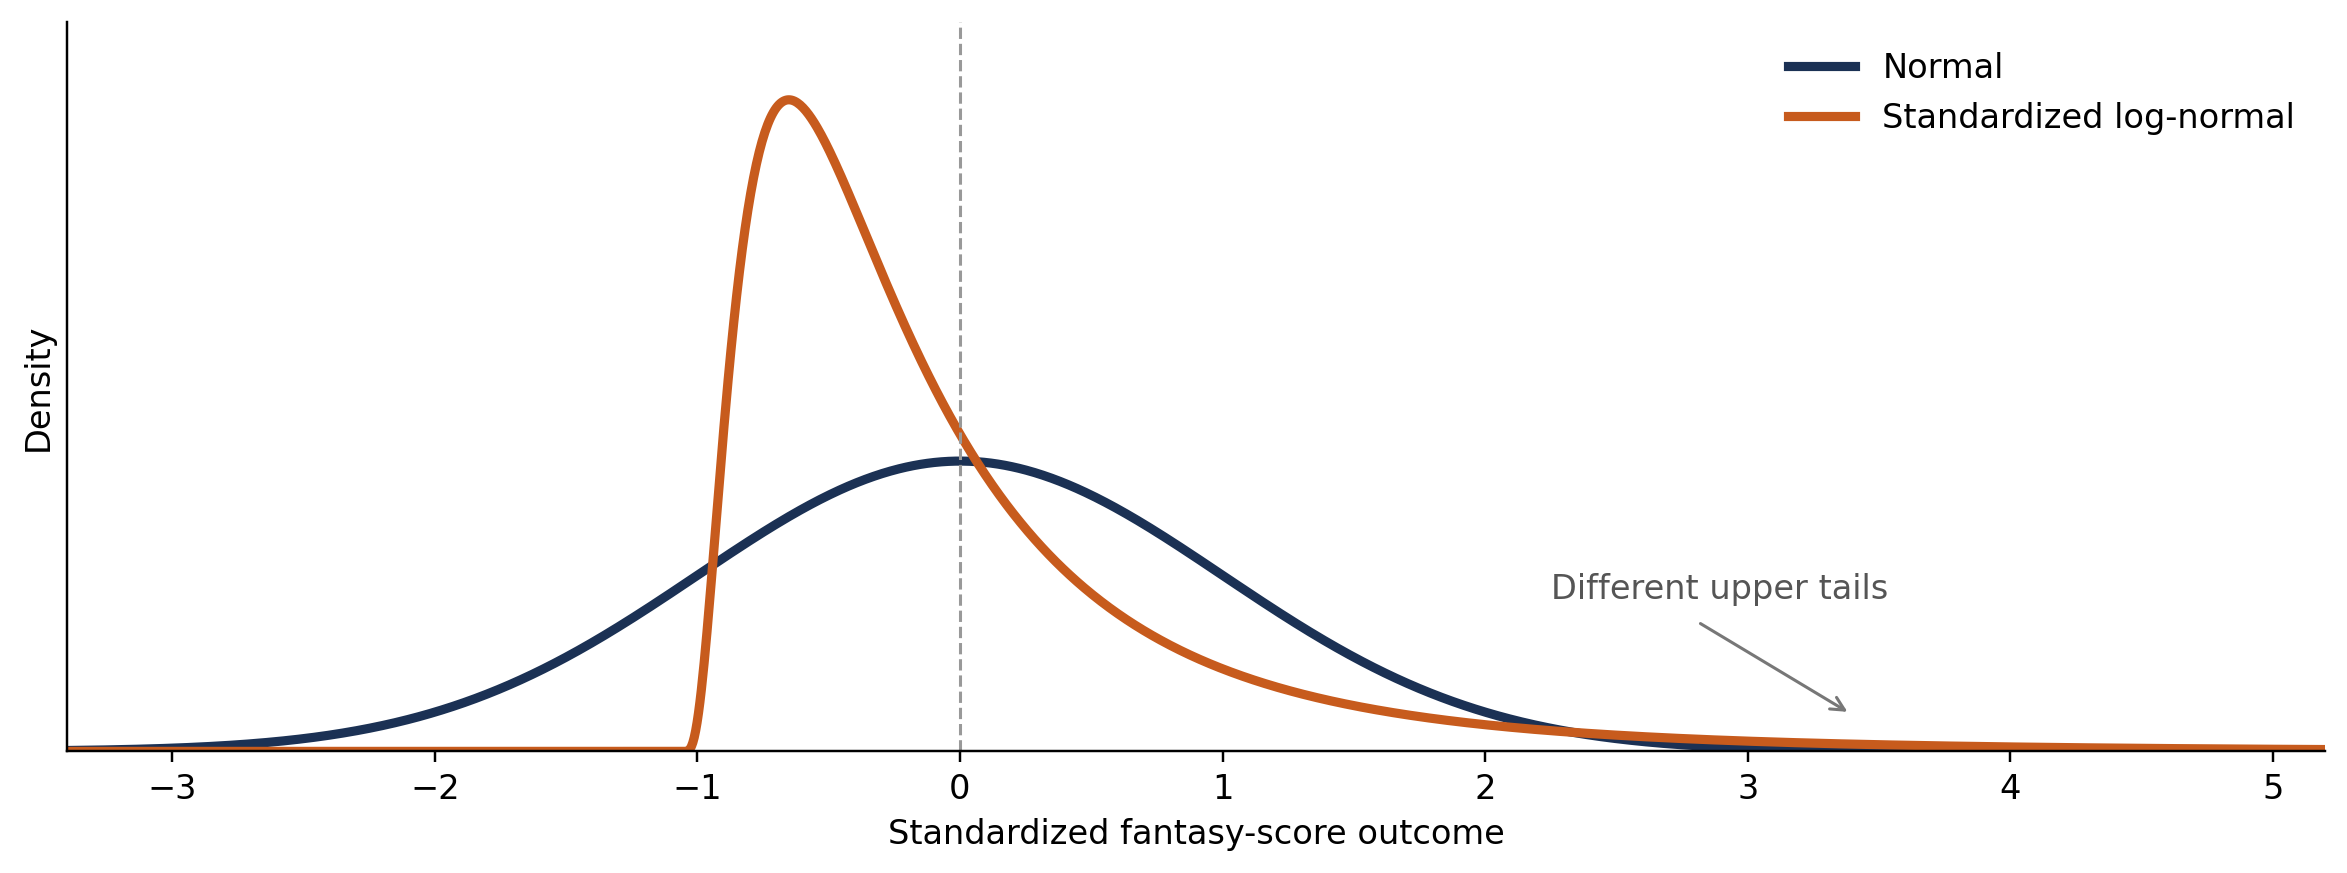
\includegraphics[width=\textwidth]{skewness_normal_vs_lognormal}\\[2pt]
      {\scriptsize Normal vs.\ standardized lognormal ($\sigma_{\log} = 0.8$): both have
      mean 0 and variance 1.\par}
    \end{column}
  \end{columns}
\end{frame}

% ====================================================================== 7
\begin{frame}{Result 1: the contest simulator matches theory}
  A lineup drawn from the field is interchangeable with every opponent, so its expected
  return must be exactly the rake: $\E[\text{payout}] = (1 - 0.15) \times \$1$.
  \vspace{0.6em}
  \begin{columns}[c]
    \begin{column}{0.36\textwidth}
      \bigstat{$-15.9\,\%$}{simulated ROI, 95\,\% CI $-19.0\,\%$ to $-12.8\,\%$
      (theory $-15\,\%$), 400{,}000 held-out entries}
      \vspace{1.2em}

      \bigstat{19.9\,\%}{cash rate (theory 20\,\%); top-0.1\,\% rate 0.10\,\% (theory
      0.10\,\%)}
    \end{column}
    \begin{column}{0.62\textwidth}
      \centering
      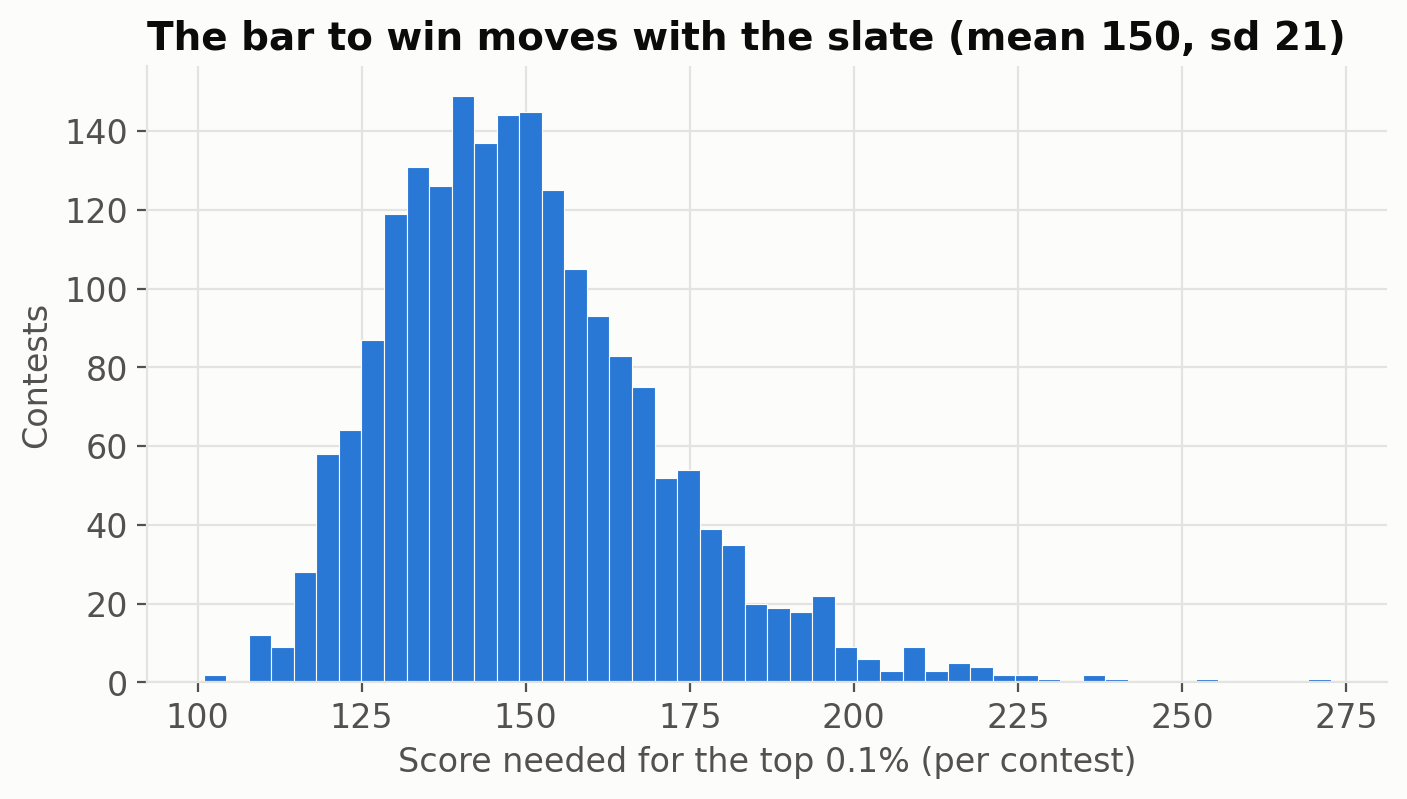
\includegraphics[width=\textwidth]{cutoff_distribution}
      {\footnotesize The winning line moves from contest to contest (mean 150, SD 21), so it
      must be simulated, not fixed.\par}
    \end{column}
  \end{columns}
  \vfill
  {\scriptsize\color{navy} All CIs are clustered by simulated field (200 fields $\times$ 10
  outcome draws).\par}
\end{frame}

% ====================================================================== 8
\begin{frame}{Result 2: field-aware upside wins the top spots}
  \centering
  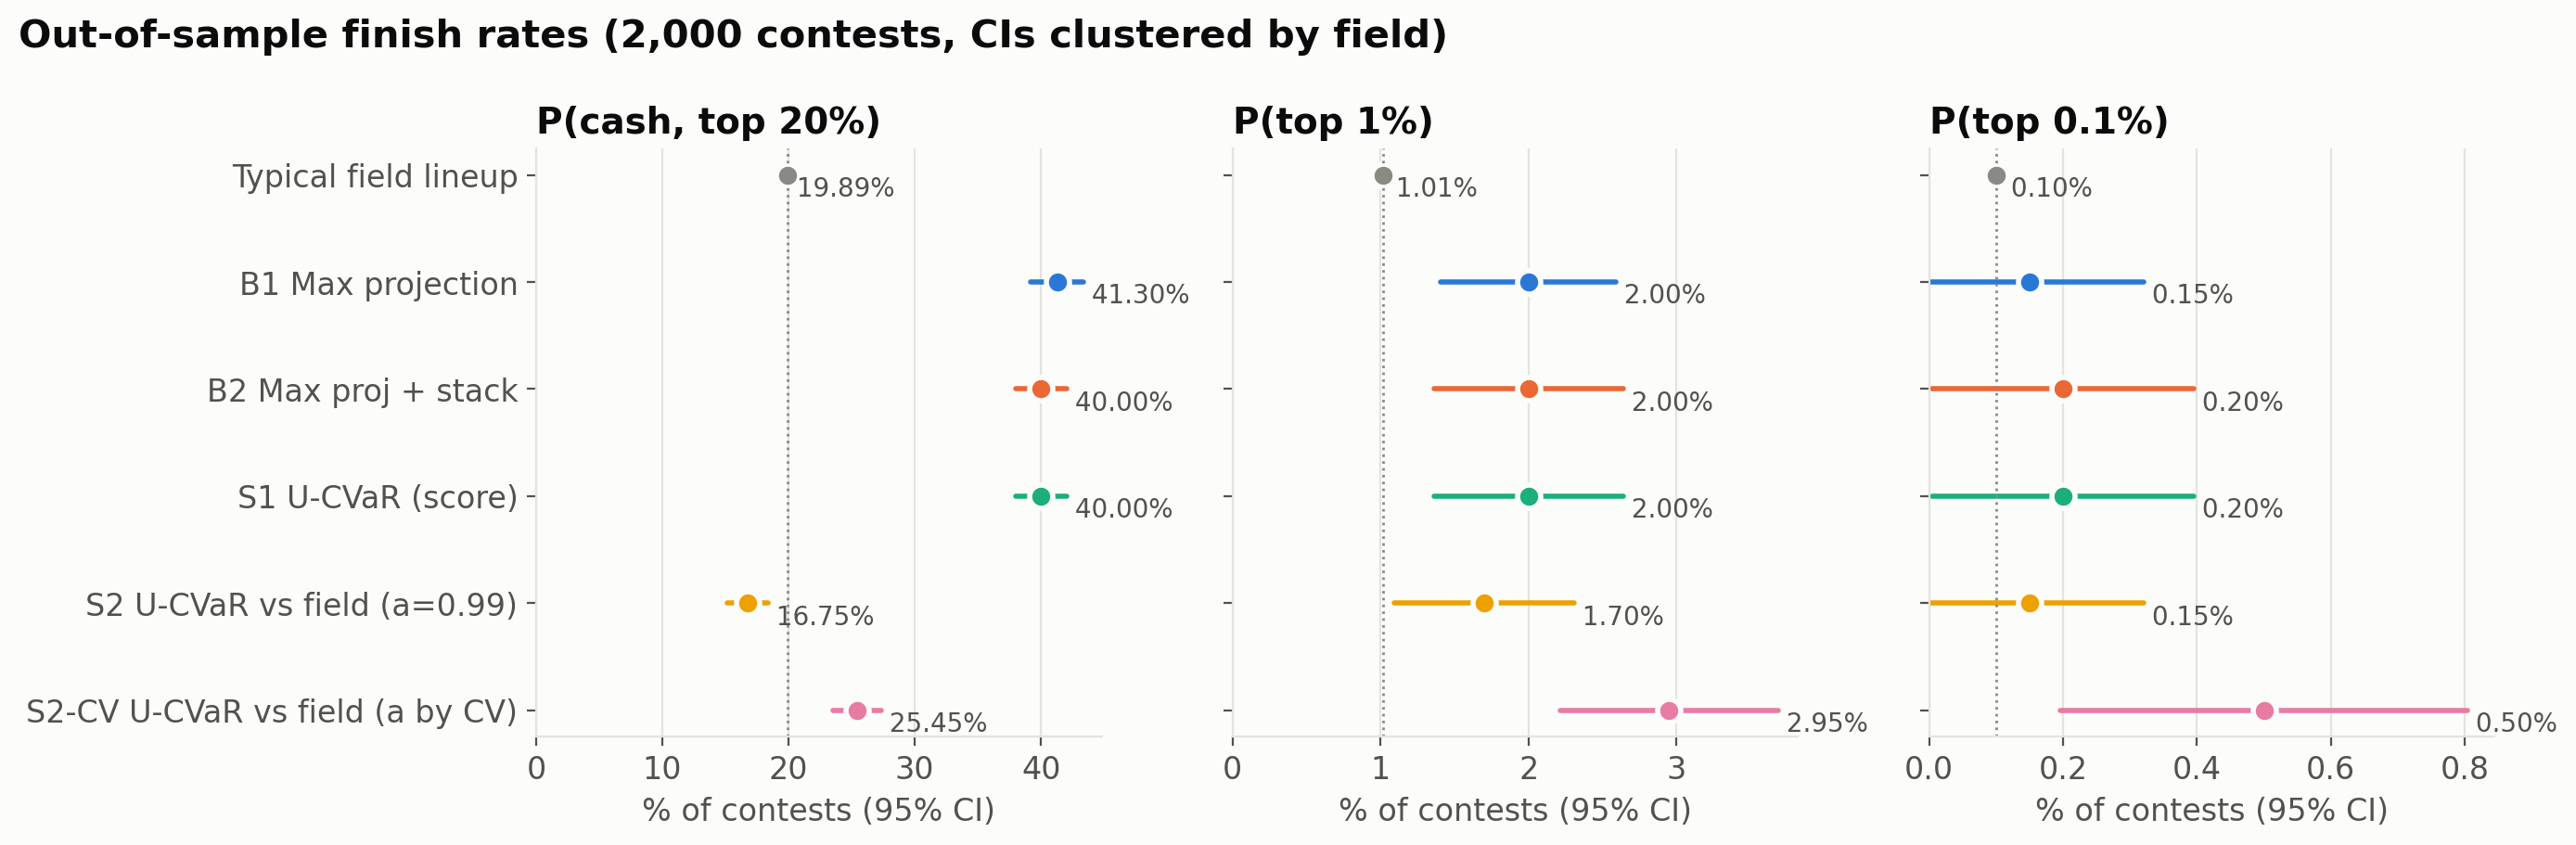
\includegraphics[width=0.92\textwidth]{results_finish_rates}
  \begin{itemize}
    \small
    \item Upside on \emph{points alone} just picks the obvious QB--WR stack: no edge
    \item \hl{Field-aware U-CVaR} ($\alpha$ chosen by validation) vs.\ max projection
      (paired): top 1\,\% $+0.95$ pts ($p = 0.04$), top 0.1\,\% $+0.35$ pts
      ($p = 0.052$), cashes 16 pts less often; top-0.1\,\% rate 5$\times$ the field's
      ($p = 0.01$)
    \item The lineup is a \emph{game stack}: one team's QB, RB, WR1 plus the opponent's WR1
  \end{itemize}
\end{frame}

% ====================================================================== 9
\begin{frame}{Result 3: choosing on the far tail over-fits}
  \begin{columns}[c]
    \begin{column}{0.52\textwidth}
      \centering
      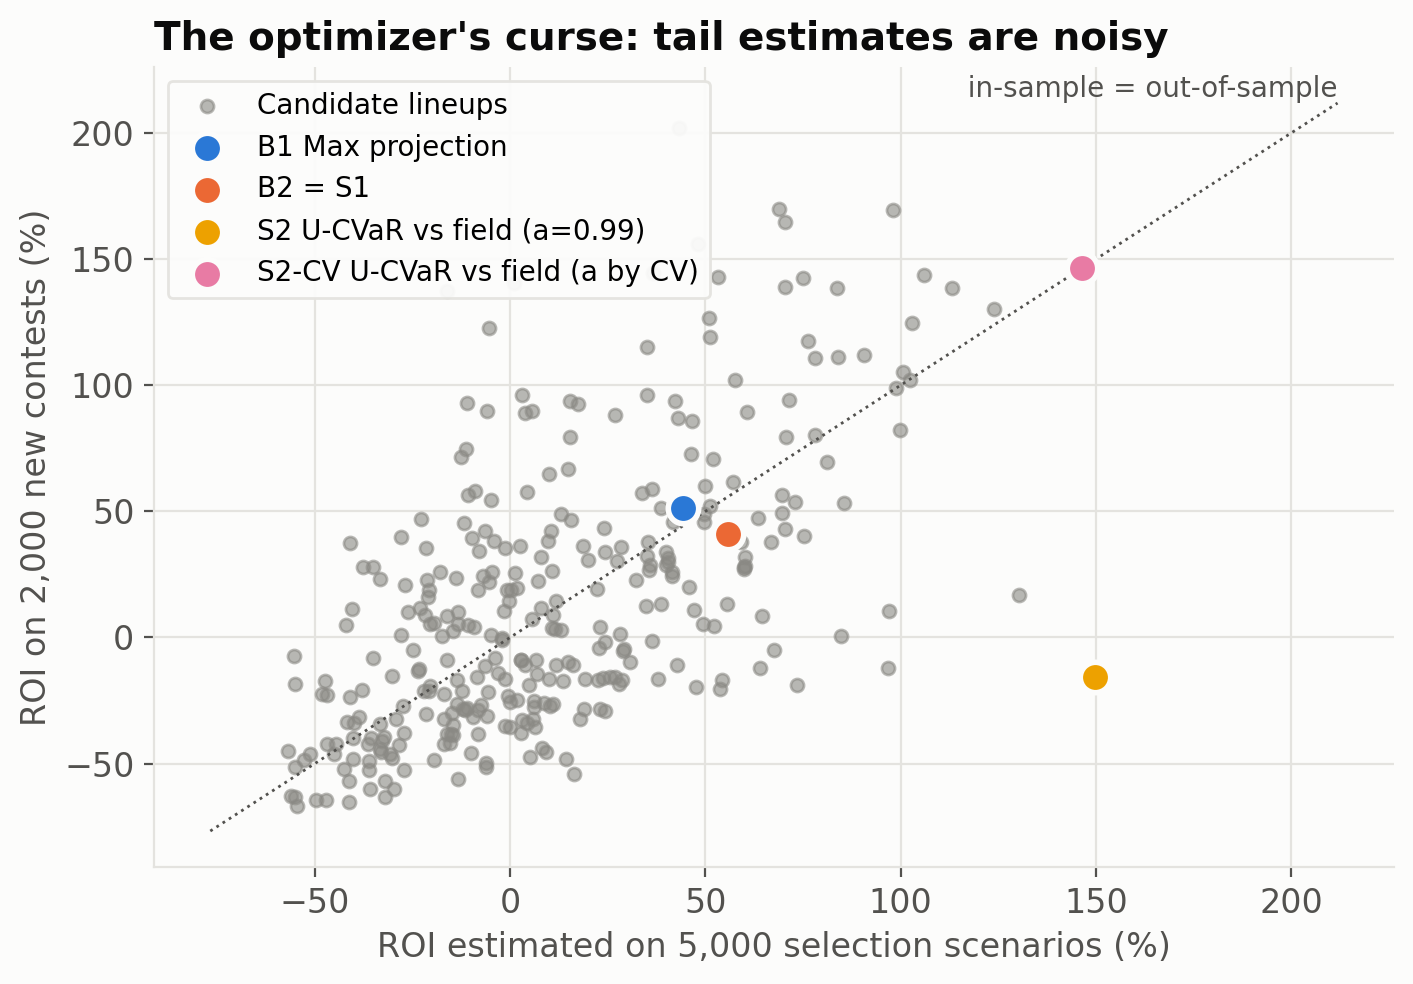
\includegraphics[width=\textwidth]{optimizers_curse}
    \end{column}
    \begin{column}{0.46\textwidth}
      \centering\small
      {\footnotesize\begin{tabular}{@{}lrr@{}}
        \toprule
        Lineup & Est.\ ROI & Test ROI \\
        \midrule
        Max projection & $+44\,\%$ & $+51\,\%$ \\
        U-CVaR, $\alpha = 0.99$ & $+150\,\%$ & \textcolor{warn}{$-16\,\%$} \\
        U-CVaR, validated $\alpha$ & $+146\,\%$ & \textcolor{good}{$+146\,\%$} \\
        \bottomrule
      \end{tabular}}
      \vspace{0.8em}
      \begin{itemize}
        \setlength\itemsep{0.3em}
        \item The 0.99 tail is only 50 scenarios
        \item \hl{Fix:} pick $\alpha$ on half the selection fields, check on the other half;
          test set never touched
        \item Payout gap vs.\ max projection: $+95$ pts, CI $[-17, +236]$, $p = 0.15$:
          \hl{not significant yet}
      \end{itemize}
    \end{column}
  \end{columns}
\end{frame}

% ====================================================================== 10
\begin{frame}{Result 4: importance sampling makes the tail cheaper}
  \begin{columns}[c]
    \begin{column}{0.47\textwidth}
      Estimate $p = P(\text{lineup score} > c)$. Draw $Z \sim N(\theta, R)$, tilted toward
      our lineup's players, and weight each draw by
      \[
        L(Z) = \frac{\varphi(Z;\,0,R)}{\varphi(Z;\,\theta,R)}
      \]
      \vspace{-0.4em}
      \begin{itemize}
        \setlength\itemsep{0.4em}
        \item \hl{8$\times$ fewer samples} for the same accuracy: IS with 250 draws matches
          crude MC with 2{,}000
        \item Gain grows as the event gets rarer: \hl{6$\times$ to 21$\times$}
      \end{itemize}
    \end{column}
    \begin{column}{0.51\textwidth}
      \centering
      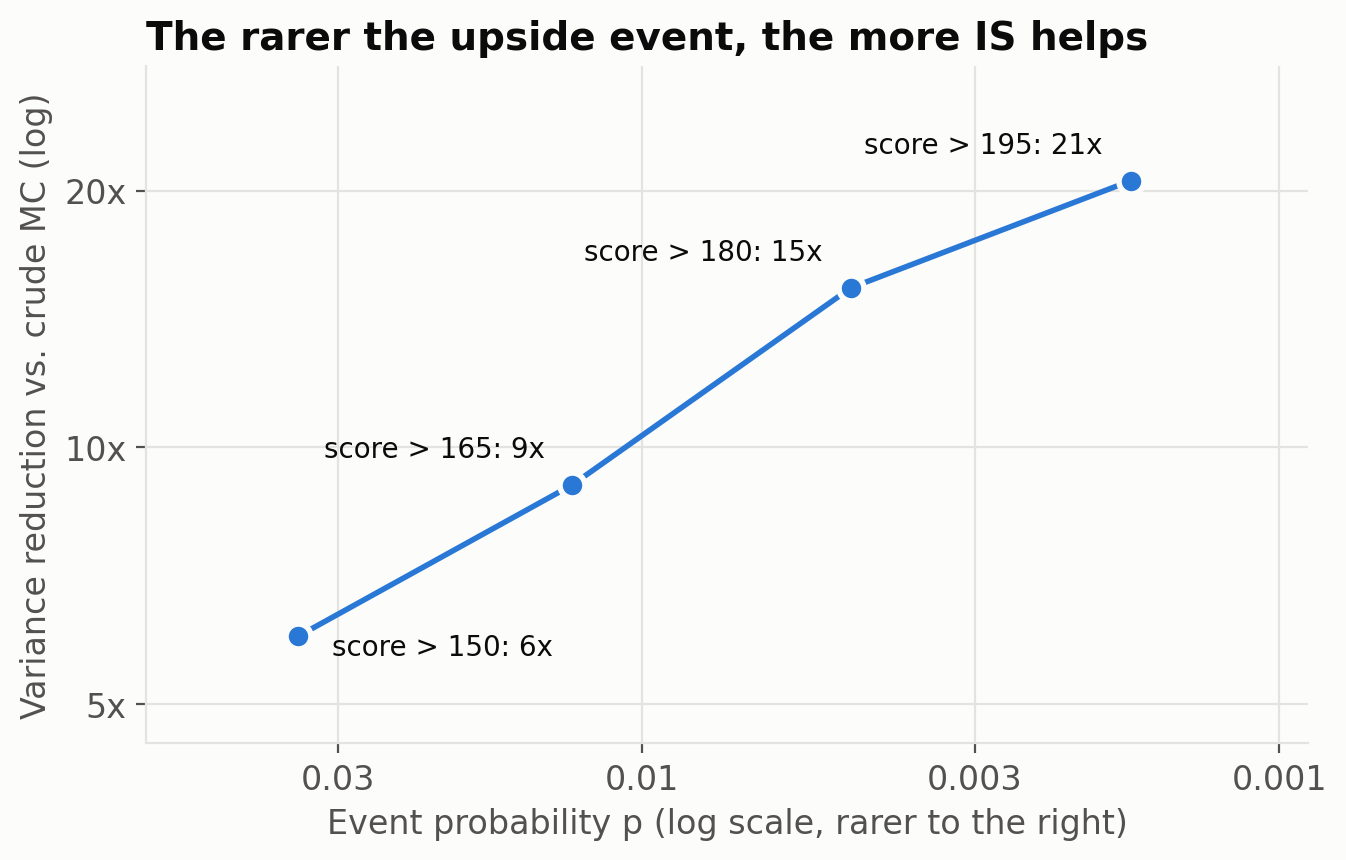
\includegraphics[width=\textwidth]{is_thresholds}
    \end{column}
  \end{columns}
\end{frame}

% ====================================================================== 11
\begin{frame}{Next steps (final report due Dec 9)}
  \centering\small
  \begin{tabular}{@{}lp{0.72\textwidth}@{}}
    \toprule
    When & What \\
    \midrule
    Nov 25--30 & Real DraftKings slate; fitted distributions and correlations \\
    Nov 27--Dec 2 & Fitted ownership model; larger field (toward 100k) \\
    Nov 28--Dec 3 & Mean--CVaR candidates; multi-entry portfolios vs.\ the paper \\
    Nov 30--Dec 4 & Importance sampling \emph{inside} selection; more contests \\
    Dec 2--9 & Sensitivity ($\alpha$, stacking, field size, payouts); final report \\
    \bottomrule
  \end{tabular}
  \vspace{0.9em}

  \raggedright
  {\footnotesize \textbf{Not shown yet:} synthetic slate; 10k field, not 100k+; single
  entry; wide payout CIs.\par}
  \vspace{0.4em}
  \textbf{Goal:} show whether the field-aware edge in expected payout becomes statistically
  significant.
\end{frame}

% ====================================================================== 12
\begin{frame}{Takeaways}
  \begin{itemize}
    \setlength\itemsep{0.8em}
    \item A three-stage contest simulator that \hl{reproduces the $-15\,\%$ rake} for a
      typical entry
    \item Upside measured \hl{against the simulated field} finds a low-owned game stack that
      reaches the top 1\,\% and top 0.1\,\% more often than max projection
    \item The far tail over-fits; validating $\alpha$ fixes it, and \hl{importance
      sampling} (up to 21$\times$) will make the tail estimates precise
  \end{itemize}
  \vfill
  \centering{\LARGE\bfseries\color{navy} Questions?}
  \vfill
\end{frame}

\end{document}
